\documentclass[aspectratio=169,10pt]{beamer}

\usetheme{Madrid}
\usecolortheme{default}
\usefonttheme{professionalfonts}
\setbeamertemplate{navigation symbols}{}
\setbeamertemplate{blocks}[rounded][shadow=false]

\usepackage{amsmath,amssymb}
\usepackage{booktabs}
\usepackage{tabularx}
\usepackage{array}
\usepackage{colortbl}
\usepackage{tikz}
\usetikzlibrary{arrows.meta,calc,fit,positioning,shapes.geometric}
\usepackage{ragged2e}
\usepackage{hyperref}
\usepackage{graphicx}
\graphicspath{{./}{slide/}}

\definecolor{PrismNavy}{HTML}{0F172A}
\definecolor{PrismBlue}{HTML}{2563EB}
\definecolor{PrismTeal}{HTML}{0F766E}
\definecolor{PrismGold}{HTML}{B45309}
\definecolor{PrismSky}{HTML}{0EA5E9}
\definecolor{PrismSlate}{HTML}{475569}
\definecolor{PrismInk}{HTML}{111827}
\definecolor{PrismMist}{HTML}{F8FAFC}
\definecolor{PrismRed}{HTML}{B91C1C}

\setbeamercolor{normal text}{fg=PrismInk,bg=white}
\setbeamercolor{title}{fg=PrismNavy}
\setbeamercolor{subtitle}{fg=PrismSlate}
\setbeamercolor{frametitle}{fg=PrismNavy,bg=white}
\setbeamercolor{structure}{fg=PrismBlue}
\setbeamercolor{block title}{fg=PrismNavy,bg=PrismBlue!12}
\setbeamercolor{block body}{fg=PrismInk,bg=PrismBlue!4}
\setbeamercolor{exampleblock title}{fg=PrismNavy,bg=PrismTeal!14}
\setbeamercolor{exampleblock body}{fg=PrismInk,bg=PrismTeal!5}
\setbeamercolor{alertblock title}{fg=PrismNavy,bg=PrismGold!20}
\setbeamercolor{alertblock body}{fg=PrismInk,bg=PrismGold!8}
\setbeamercolor{author in head/foot}{fg=white,bg=PrismNavy}
\setbeamercolor{title in head/foot}{fg=white,bg=PrismBlue}
\setbeamercolor{date in head/foot}{fg=white,bg=PrismNavy}

\setbeamertemplate{headline}{}
\setbeamertemplate{footline}{%
  \leavevmode%
  \hbox{%
    \begin{beamercolorbox}[wd=.50\paperwidth,ht=2.9ex,dp=1.2ex,leftskip=0.8em]{author in head/foot}%
      \usebeamerfont{author in head/foot}\insertshortauthor
    \end{beamercolorbox}%
    \begin{beamercolorbox}[wd=.30\paperwidth,ht=2.9ex,dp=1.2ex,center]{title in head/foot}%
      \usebeamerfont{title in head/foot}\insertshorttitle
    \end{beamercolorbox}%
    \begin{beamercolorbox}[wd=.20\paperwidth,ht=2.9ex,dp=1.2ex,rightskip=1em plus 1fil]{date in head/foot}%
      \usebeamerfont{date in head/foot}\insertshortdate{}\hspace*{1.3em}\insertframenumber/\inserttotalframenumber
    \end{beamercolorbox}%
  }%
}

\setbeamerfont{title}{size=\Huge,series=\bfseries}
\setbeamerfont{frametitle}{size=\Large,series=\bfseries}
\setbeamerfont{block title}{series=\bfseries}
\setbeamerfont{author in head/foot}{size=\tiny}
\setbeamerfont{title in head/foot}{size=\tiny}
\setbeamerfont{date in head/foot}{size=\tiny}

\newcolumntype{Y}{>{\RaggedRight\arraybackslash}X}

\newcommand{\pill}[2]{%
  \tikz[baseline=-0.55ex]\node[
    fill=#1!15,
    draw=#1!35,
    text=#1,
    rounded corners=3pt,
    inner xsep=6pt,
    inner ysep=2.5pt
  ]{\scriptsize\bfseries #2};%
}

\newcommand{\source}[1]{%
  % Intentionally hidden in the presentation deck.
}

\newcommand{\metric}[3]{%
  \begin{beamercolorbox}[wd=\textwidth,rounded=true,sep=0.55em]{#1}
    {\scriptsize\color{PrismSlate}#2}\par
    {\Large\bfseries #3}
  \end{beamercolorbox}
}

\newcommand{\chartbar}[5]{%
  \node[anchor=east] at (0,#1) {\scriptsize #2};
  \fill[#3] (0.15,#1-0.11) rectangle (#4,#1+0.11);
  \node[anchor=west] at (#4+0.10,#1) {\scriptsize #5};
}

\newcommand{\screenshotframe}[2]{%
  \begin{frame}{#1}
    \centering
    \vspace{-0.08cm}
    \begingroup
    \setlength{\fboxsep}{0pt}
    \setlength{\fboxrule}{0.35pt}
    \color{PrismSlate!35}
    \fbox{%
      \includegraphics[
        width=0.985\textwidth,
        height=0.78\textheight,
        keepaspectratio
      ]{screenshots/#2}%
    }%
    \endgroup
  \end{frame}
}

\title[TryOps MLOps]{TryOps: Enterprise MLOps for Governed VTON and Efficient LLM Serving}
\subtitle{Evidence Gates, Native Control Plane, and Measured Optimization Results}
\author[Nguyen Tran Nhat Trung, Hoang Minh Thai, Pham Hai Dang]{Nguyen Tran Nhat Trung\ (23521684) \and Hoang Minh Thai\ (23521414) \and Pham Hai Dang\ (23520233)}
\date[June 2026]{June 2026}

\begin{document}

\begin{frame}
  \vspace{0.08cm}
  {\LARGE\bfseries\color{PrismNavy}\inserttitle\par}
  \vspace{0.08cm}
  {\large\color{PrismSlate}\insertsubtitle\par}
  \vspace{0.10cm}
  {\scriptsize\color{PrismSlate}
    Nguyen Tran Nhat Trung (23521684)\hspace{0.35cm}
    Hoang Minh Thai (23521414)\hspace{0.35cm}
    Pham Hai Dang (23520233)\par}
  \vspace{0.20cm}

  \pill{PrismBlue}{VTON}\hspace{0.18cm}
  \pill{PrismTeal}{LLM Pareto}\hspace{0.18cm}
  \pill{PrismGold}{Policy gates}\hspace{0.18cm}
  \pill{PrismSky}{Native boundary}\hspace{0.18cm}
  \pill{PrismRed}{Energy}

  \vspace{0.24cm}
  \begin{columns}[T,totalwidth=\textwidth]
    \column{0.58\textwidth}
    \begin{itemize}\itemsep0.20em
      \item TryOps treats models as governed production assets, not notebook outputs.
      \item The same spine runs offline contracts and real GPU backends behind unchanged APIs.
      \item VTON and optimized LLM serving stress different failure modes: visual quality, latency, VRAM, cost, energy, rollback, and auditability.
    \end{itemize}

    \column{0.38\textwidth}
    \begin{beamercolorbox}[wd=\textwidth,rounded=true,sep=0.75em]{exampleblock body}
      \textbf{Executive claim}\par
      No model reaches users without evaluation evidence, a policy gate, and traceable lineage.
    \end{beamercolorbox}
  \end{columns}

  \source{\texttt{README.md}; \texttt{reports/final\_report.md}; \texttt{docs/presentation\_outline.md}.}
\end{frame}

\begin{frame}{The Production ML Problem}
  \small
  \begin{columns}[T,totalwidth=\textwidth]
    \column{0.49\textwidth}
    \begin{block}{The demo is the easy part}
      A model can generate a plausible output while still being impossible to reproduce, monitor, secure, roll back, or compare against a previous version.
    \end{block}

    \begin{alertblock}{What breaks in production}
      \begin{itemize}\itemsep0.24em
        \item No data, code, config, or hardware lineage
        \item Manual promotion decisions with weak evidence
        \item SLOs calibrated to the wrong backend
        \item Optimization claims that ignore energy and cost
      \end{itemize}
    \end{alertblock}

    \column{0.47\textwidth}
    \begin{exampleblock}{TryOps answer}
      Build a reproducible control plane where every candidate flows through versioned inputs, tracked runs, native evaluation, policy-as-code, signed promotion evidence, monitoring, and rollback.
    \end{exampleblock}

    \begin{beamercolorbox}[wd=\textwidth,rounded=true,sep=0.9em]{block body}
      \textbf{Research question}\par
      What architecture makes VTON and optimized LLM systems reproducible, governable, measurable, and continuously deployable?
    \end{beamercolorbox}
  \end{columns}
  \source{\texttt{reports/final\_report.md}, Sections 1--4.}
\end{frame}

\begin{frame}{Thesis and Workloads}
  \small
  \begin{columns}[T,totalwidth=\textwidth]
    \column{0.48\textwidth}
    \begin{block}{VTON: visual and GPU-heavy}
      Person image + garment image \(\rightarrow\) generated try-on result. The hard parts are quality measurement, artifact lineage, privacy, quota, fallback behavior, and visual failure analysis.
    \end{block}

    \begin{exampleblock}{Evidence in repo}
      Deterministic baseline, real SD1.5 inpainting sample, native image metrics, VTON advanced evaluation, comparison gallery, and blocked bad-candidate release evidence.
    \end{exampleblock}

    \column{0.48\textwidth}
    \begin{block}{LLM optimization: latency and memory-bound}
      Quantization, batching, and serving controls are judged by quality, p95 latency, throughput, VRAM, energy, carbon, and rollback risk.
    \end{block}

    \begin{exampleblock}{Evidence in repo}
      Real SmolLM2 inference, Qwen2.5 fp16/8-bit/4-bit Pareto sweep, native C++ SLO gate, energy/carbon sweep, leaderboard, and continuous-batching simulator.
    \end{exampleblock}
  \end{columns}

  \begin{alertblock}{Thesis}
    MLOps is the product. Models are governed assets that must earn promotion.
  \end{alertblock}
  \source{\texttt{docs/architecture.md}; \texttt{reports/benchmark\_run\_report.md}.}
\end{frame}

\begin{frame}{Architecture: Product Boundary}
  \scriptsize
  \centering
  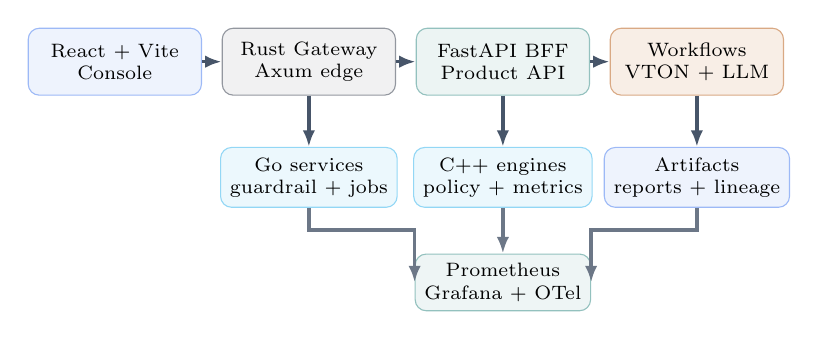
\begin{tikzpicture}[node distance=0.25cm, every node/.style={font=\scriptsize}]
    \node[draw=PrismBlue!45, fill=PrismBlue!8, rounded corners=4pt, minimum width=2.2cm, minimum height=0.85cm, align=center] (web) {React + Vite\\Console};
    \node[draw=PrismNavy!45, fill=PrismNavy!6, rounded corners=4pt, minimum width=2.2cm, minimum height=0.85cm, align=center, right=of web] (gateway) {Rust Gateway\\Axum edge};
    \node[draw=PrismTeal!45, fill=PrismTeal!8, rounded corners=4pt, minimum width=2.2cm, minimum height=0.85cm, align=center, right=of gateway] (api) {FastAPI BFF\\Product API};
    \node[draw=PrismGold!50, fill=PrismGold!10, rounded corners=4pt, minimum width=2.2cm, minimum height=0.85cm, align=center, right=of api] (workflows) {Workflows\\VTON + LLM};

    \node[draw=PrismSky!45, fill=PrismSky!8, rounded corners=4pt, minimum width=2.0cm, minimum height=0.76cm, align=center, below=0.65cm of gateway] (go) {Go services\\guardrail + jobs};
    \node[draw=PrismSky!45, fill=PrismSky!8, rounded corners=4pt, minimum width=2.0cm, minimum height=0.76cm, align=center, below=0.65cm of api] (cpp) {C++ engines\\policy + metrics};
    \node[draw=PrismBlue!45, fill=PrismBlue!8, rounded corners=4pt, minimum width=2.0cm, minimum height=0.76cm, align=center, below=0.65cm of workflows] (store) {Artifacts\\reports + lineage};

    \node[draw=PrismTeal!45, fill=PrismTeal!7, rounded corners=4pt, minimum width=2.2cm, minimum height=0.72cm, align=center, below=0.58cm of cpp] (obs) {Prometheus\\Grafana + OTel};

    \draw[-{Latex[length=2.1mm]}, very thick, PrismSlate] (web) -- (gateway);
    \draw[-{Latex[length=2.1mm]}, very thick, PrismSlate] (gateway) -- (api);
    \draw[-{Latex[length=2.1mm]}, very thick, PrismSlate] (api) -- (workflows);
    \draw[-{Latex[length=2.1mm]}, very thick, PrismSlate] (gateway) -- (go);
    \draw[-{Latex[length=2.1mm]}, very thick, PrismSlate] (api) -- (cpp);
    \draw[-{Latex[length=2.1mm]}, very thick, PrismSlate] (workflows) -- (store);
    \draw[-{Latex[length=2.1mm]}, very thick, PrismSlate!80] (go.south) -- ++(0,-0.28) -| (obs.west);
    \draw[-{Latex[length=2.1mm]}, very thick, PrismSlate!80] (cpp.south) -- (obs.north);
    \draw[-{Latex[length=2.1mm]}, very thick, PrismSlate!80] (store.south) -- ++(0,-0.28) -| (obs.east);
  \end{tikzpicture}

  \vspace{0.25cm}
  \begin{columns}[T,totalwidth=\textwidth]
    \column{0.48\textwidth}
    \begin{block}{Compiled production boundary}
      Rust fronts \texttt{/api/*}; Go owns sidecars, controller-style services, and native drivers; C++ carries deterministic hot-path engines.
    \end{block}
    \column{0.48\textwidth}
    \begin{exampleblock}{Python role}
      Python coordinates ML workflows and product APIs, while risk-critical decisions are mirrored or moved into native tools with graceful fallback.
    \end{exampleblock}
  \end{columns}
  \source{\texttt{README.md}; \texttt{docs/adr/0003-native-production-boundary.md}; \texttt{docs/architecture.md}.}
\end{frame}

\begin{frame}{Request Flow: Console to Evidence}
  \scriptsize
  \centering
  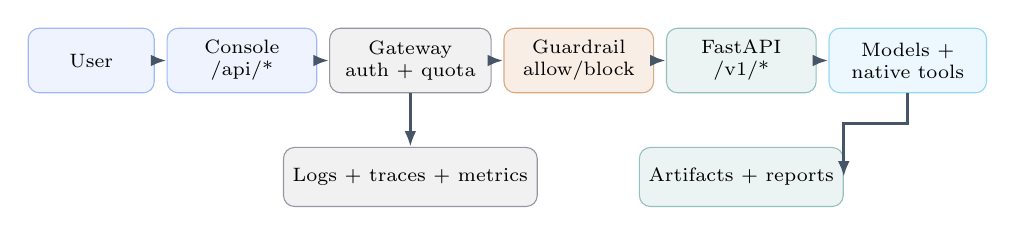
\begin{tikzpicture}[node distance=0.15cm, every node/.style={font=\scriptsize}]
    \node[draw=PrismBlue!45, fill=PrismBlue!8, rounded corners=4pt, minimum width=1.6cm, minimum height=0.82cm, align=center] (user) {User};
    \node[draw=PrismBlue!45, fill=PrismBlue!8, rounded corners=4pt, minimum width=1.9cm, minimum height=0.82cm, align=center, right=of user] (console) {Console\\/api/*};
    \node[draw=PrismNavy!45, fill=PrismNavy!6, rounded corners=4pt, minimum width=2.05cm, minimum height=0.82cm, align=center, right=of console] (gateway) {Gateway\\auth + quota};
    \node[draw=PrismGold!50, fill=PrismGold!10, rounded corners=4pt, minimum width=1.9cm, minimum height=0.82cm, align=center, right=of gateway] (guardrail) {Guardrail\\allow/block};
    \node[draw=PrismTeal!45, fill=PrismTeal!8, rounded corners=4pt, minimum width=1.9cm, minimum height=0.82cm, align=center, right=of guardrail] (api) {FastAPI\\/v1/*};
    \node[draw=PrismSky!45, fill=PrismSky!8, rounded corners=4pt, minimum width=2.0cm, minimum height=0.82cm, align=center, right=of api] (models) {Models +\\native tools};

    \node[draw=PrismTeal!45, fill=PrismTeal!8, rounded corners=4pt, minimum width=2.35cm, minimum height=0.75cm, align=center, below=0.68cm of api] (evidence) {Artifacts + reports};
    \node[draw=PrismNavy!45, fill=PrismNavy!6, rounded corners=4pt, minimum width=2.35cm, minimum height=0.75cm, align=center, below=0.68cm of gateway] (obs) {Logs + traces + metrics};

    \draw[-{Latex[length=2mm]}, very thick, PrismSlate] (user) -- (console);
    \draw[-{Latex[length=2mm]}, very thick, PrismSlate] (console) -- (gateway);
    \draw[-{Latex[length=2mm]}, very thick, PrismSlate] (gateway) -- (guardrail);
    \draw[-{Latex[length=2mm]}, very thick, PrismSlate] (guardrail) -- (api);
    \draw[-{Latex[length=2mm]}, very thick, PrismSlate] (api) -- (models);
    \draw[-{Latex[length=2mm]}, very thick, PrismSlate] (models.south) -- ++(0,-0.38) -| (evidence.east);
    \draw[-{Latex[length=2mm]}, very thick, PrismSlate] (gateway.south) -- (obs.north);
  \end{tikzpicture}

  \vspace{0.25cm}
  \begin{columns}[T,totalwidth=\textwidth]
    \column{0.49\textwidth}
    \begin{block}{Edge responsibilities}
      API-key and token checks, request IDs, rate and body limits, quota admission, semantic-cache admission, edge guardrail calls, metrics, and proxying.
    \end{block}
    \column{0.47\textwidth}
    \begin{exampleblock}{Workflow responsibilities}
      VTON, LLM, evaluation, governance, promotion, rollback, and evidence writes under reproducible run context.
    \end{exampleblock}
  \end{columns}
  \source{\texttt{README.md}; \texttt{docs/api\_contract.md}; \texttt{docs/opentelemetry\_tracing.md}.}
\end{frame}

\begin{frame}{Port Surface: Ingress, Not Open Backends}
  \scriptsize
  \centering
  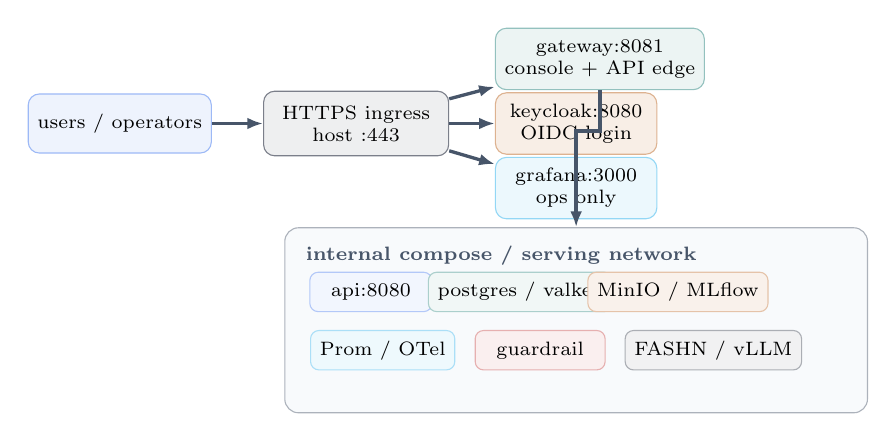
\begin{tikzpicture}[node distance=0.28cm, every node/.style={font=\scriptsize}]
    \node[draw=PrismBlue!45, fill=PrismBlue!8, rounded corners=4pt, minimum width=2.25cm, minimum height=0.75cm, align=center] (users) {users / operators};
    \node[draw=PrismNavy!55, fill=PrismNavy!7, rounded corners=4pt, minimum width=2.35cm, minimum height=0.82cm, align=center, right=0.65cm of users] (ingress) {HTTPS ingress\\host :443};

    \node[draw=PrismTeal!45, fill=PrismTeal!8, rounded corners=4pt, minimum width=2.05cm, minimum height=0.78cm, align=center, right=0.58cm of ingress, yshift=0.82cm] (gateway) {gateway:8081\\console + API edge};
    \node[draw=PrismGold!45, fill=PrismGold!10, rounded corners=4pt, minimum width=2.05cm, minimum height=0.78cm, align=center, right=0.58cm of ingress] (keycloak) {keycloak:8080\\OIDC login};
    \node[draw=PrismSky!45, fill=PrismSky!8, rounded corners=4pt, minimum width=2.05cm, minimum height=0.78cm, align=center, right=0.58cm of ingress, yshift=-0.82cm] (grafana) {grafana:3000\\ops only};

    \node[draw=PrismSlate!45, fill=PrismMist, rounded corners=5pt, minimum width=7.4cm, minimum height=2.35cm, align=center, below=0.92cm of keycloak] (internal) {};
    \node[anchor=north west, text=PrismSlate] at ($(internal.north west)+(0.15,-0.12)$) {\bfseries internal compose / serving network};
    \node[draw=PrismBlue!35, fill=PrismBlue!6, rounded corners=3pt, minimum width=1.55cm, minimum height=0.50cm, align=center] at ($(internal.west)+(1.1,0.36)$) {api:8080};
    \node[draw=PrismTeal!35, fill=PrismTeal!6, rounded corners=3pt, minimum width=1.7cm, minimum height=0.50cm, align=center] at ($(internal.west)+(3.0,0.36)$) {postgres / valkey};
    \node[draw=PrismGold!35, fill=PrismGold!8, rounded corners=3pt, minimum width=1.7cm, minimum height=0.50cm, align=center] at ($(internal.west)+(5.0,0.36)$) {MinIO / MLflow};
    \node[draw=PrismSky!35, fill=PrismSky!7, rounded corners=3pt, minimum width=1.75cm, minimum height=0.50cm, align=center] at ($(internal.west)+(1.25,-0.38)$) {Prom / OTel};
    \node[draw=PrismRed!35, fill=PrismRed!7, rounded corners=3pt, minimum width=1.65cm, minimum height=0.50cm, align=center] at ($(internal.west)+(3.25,-0.38)$) {guardrail};
    \node[draw=PrismNavy!35, fill=PrismNavy!6, rounded corners=3pt, minimum width=2.15cm, minimum height=0.50cm, align=center] at ($(internal.west)+(5.45,-0.38)$) {FASHN / vLLM};

    \draw[-{Latex[length=2mm]}, very thick, PrismSlate] (users) -- (ingress);
    \draw[-{Latex[length=2mm]}, very thick, PrismSlate] (ingress) -- (gateway);
    \draw[-{Latex[length=2mm]}, very thick, PrismSlate] (ingress) -- (keycloak);
    \draw[-{Latex[length=2mm]}, very thick, PrismSlate] (ingress) -- (grafana);
    \draw[-{Latex[length=2mm]}, very thick, PrismSlate] (gateway.south) -- ++(0,-0.52) -| (internal.north);
  \end{tikzpicture}

  \vspace{0.18cm}
  \begin{columns}[T,totalwidth=\textwidth]
    \column{0.48\textwidth}
    \begin{exampleblock}{Recommended shared-host surface}
      One TLS ingress routes to gateway, Keycloak, and admin-restricted Grafana. FastAPI, databases, object stores, metrics backends, guardrail, and model endpoints stay private.
    \end{exampleblock}
    \column{0.48\textwidth}
    \begin{alertblock}{Developer-local exception}
      \texttt{make app-up} exposes many convenience ports, including 18081, 18082, 13000, 15432, 19000, 15000, 19090, 4317, 4318, and 18100. That is not the shared-datacenter posture.
    \end{alertblock}
  \end{columns}
  \source{\texttt{PORT.md}, ``Shared Datacenter Port Policy'' and ``Port Relationship Chart''.}
\end{frame}

\begin{frame}{Developer-Local Port Relationship}
  \tiny
  \centering
  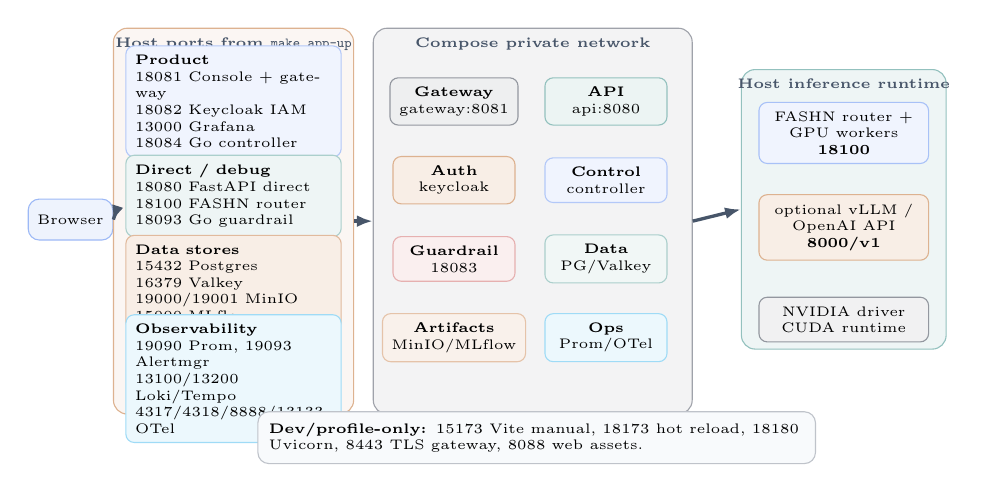
\begin{tikzpicture}[x=1cm,y=1cm, every node/.style={font=\tiny}]
    \node[draw=PrismBlue!45, fill=PrismBlue!8, rounded corners=4pt, minimum width=1.05cm, minimum height=0.52cm, align=center] (browser) at (0.38,3.05) {Browser};

    \node[draw=PrismGold!45, fill=PrismGold!5, rounded corners=5pt, minimum width=3.05cm, minimum height=4.90cm, align=center] (host) at (2.45,3.03) {};
    \node[anchor=north, text=PrismSlate] at (host.north) {\textbf{Host ports from \texttt{make app-up}}};
    \node[draw=PrismBlue!35, fill=PrismBlue!7, rounded corners=3pt, text width=2.50cm, align=left] at (2.45,4.55) {\textbf{Product}\\18081 Console + gateway\\18082 Keycloak IAM\\13000 Grafana\\18084 Go controller};
    \node[draw=PrismTeal!35, fill=PrismTeal!7, rounded corners=3pt, text width=2.50cm, align=left] at (2.45,3.35) {\textbf{Direct / debug}\\18080 FastAPI direct\\18100 FASHN router\\18093 Go guardrail};
    \node[draw=PrismGold!40, fill=PrismGold!10, rounded corners=3pt, text width=2.50cm, align=left] at (2.45,2.25) {\textbf{Data stores}\\15432 Postgres\\16379 Valkey\\19000/19001 MinIO\\15000 MLflow};
    \node[draw=PrismSky!40, fill=PrismSky!8, rounded corners=3pt, text width=2.50cm, align=left] at (2.45,1.03) {\textbf{Observability}\\19090 Prom, 19093 Alertmgr\\13100/13200 Loki/Tempo\\4317/4318/8888/13133 OTel};

    \node[draw=PrismNavy!40, fill=PrismNavy!5, rounded corners=5pt, minimum width=4.05cm, minimum height=4.90cm, align=center] (compose) at (6.25,3.03) {};
    \node[anchor=north, text=PrismSlate] at (compose.north) {\textbf{Compose private network}};
    \node[draw=PrismNavy!45, fill=PrismNavy!7, rounded corners=3pt, minimum width=1.55cm, minimum height=0.52cm, align=center] at (5.25,4.55) {\textbf{Gateway}\\gateway:8081};
    \node[draw=PrismTeal!45, fill=PrismTeal!8, rounded corners=3pt, minimum width=1.55cm, minimum height=0.52cm, align=center] at (7.18,4.55) {\textbf{API}\\api:8080};
    \node[draw=PrismGold!45, fill=PrismGold!10, rounded corners=3pt, minimum width=1.55cm, minimum height=0.52cm, align=center] at (5.25,3.55) {\textbf{Auth}\\keycloak};
    \node[draw=PrismBlue!35, fill=PrismBlue!7, rounded corners=3pt, minimum width=1.55cm, minimum height=0.52cm, align=center] at (7.18,3.55) {\textbf{Control}\\controller};
    \node[draw=PrismRed!35, fill=PrismRed!7, rounded corners=3pt, minimum width=1.55cm, minimum height=0.52cm, align=center] at (5.25,2.55) {\textbf{Guardrail}\\18083};
    \node[draw=PrismTeal!35, fill=PrismTeal!6, rounded corners=3pt, minimum width=1.55cm, minimum height=0.52cm, align=center] at (7.18,2.55) {\textbf{Data}\\PG/Valkey};
    \node[draw=PrismGold!35, fill=PrismGold!8, rounded corners=3pt, minimum width=1.55cm, minimum height=0.52cm, align=center] at (5.25,1.55) {\textbf{Artifacts}\\MinIO/MLflow};
    \node[draw=PrismSky!40, fill=PrismSky!8, rounded corners=3pt, minimum width=1.55cm, minimum height=0.52cm, align=center] at (7.18,1.55) {\textbf{Ops}\\Prom/OTel};

    \node[draw=PrismTeal!45, fill=PrismTeal!7, rounded corners=5pt, minimum width=2.60cm, minimum height=3.55cm, align=center] (runtime) at (10.20,3.18) {};
    \node[anchor=north, text=PrismSlate] at (runtime.north) {\textbf{Host inference runtime}};
    \node[draw=PrismBlue!40, fill=PrismBlue!7, rounded corners=3pt, text width=1.92cm, align=center] at (10.20,4.15) {FASHN router +\\GPU workers\\\textbf{18100}};
    \node[draw=PrismGold!45, fill=PrismGold!10, rounded corners=3pt, text width=1.92cm, align=center] at (10.20,2.95) {optional vLLM /\\OpenAI API\\\textbf{8000/v1}};
    \node[draw=PrismNavy!45, fill=PrismNavy!6, rounded corners=3pt, text width=1.92cm, align=center] at (10.20,1.78) {NVIDIA driver\\CUDA runtime};

    \node[draw=PrismSlate!35, fill=PrismMist, rounded corners=4pt, text width=6.8cm, inner sep=4pt, align=left] at (6.30,0.28) {
      \textbf{Dev/profile-only:} 15173 Vite manual, 18173 hot reload, 18180 Uvicorn, 8443 TLS gateway, 8088 web assets.
    };

    \draw[-{Latex[length=2mm]}, very thick, PrismSlate] (browser.east) -- (host.west);
    \draw[-{Latex[length=2mm]}, very thick, PrismSlate] (host.east) -- (compose.west);
    \draw[-{Latex[length=2mm]}, very thick, PrismSlate] (compose.east) -- (runtime.west);
  \end{tikzpicture}
\end{frame}

\begin{frame}{Data and Artifact Lifecycle}
  \scriptsize
  \renewcommand{\arraystretch}{1.13}
  \begin{tabularx}{\textwidth}{>{\RaggedRight\arraybackslash}p{3.1cm} Y >{\RaggedRight\arraybackslash}p{3.7cm}}
    \toprule
    \textbf{Layer} & \textbf{What TryOps records} & \textbf{Why it matters} \\
    \midrule
    Run context & Git/code version, dataset version, hardware, command, trace IDs & Reproduce any output \\
    \addlinespace
    Evaluation artifacts & LLM Pareto, energy sweep, VTON comparison, native metrics, leaderboards & Compare candidates with evidence \\
    \addlinespace
    Cards and reports & Model cards, data cards, promotion decisions, rollback records & Human-reviewable release package \\
    \addlinespace
    Lineage standards & Internal lineage plus OpenLineage validation & Audit and downstream integration \\
    \addlinespace
    Storage surfaces & Local artifacts, DVC/MinIO samples, MLflow stack surface & Versioned assets and repeatable local demos \\
    \bottomrule
  \end{tabularx}

  \vspace{0.22cm}
  \begin{alertblock}{Core invariant}
    A generated image, LLM answer, or model alias must be traceable back to input data, code, config, model version, metrics, policy verdict, and release artifact.
  \end{alertblock}
  \source{\texttt{docs/data\_versioning.md}; \texttt{docs/reproducibility\_checklist.md}; \texttt{docs/roadmap\_audit.md}.}
\end{frame}

\begin{frame}{Policy Gate: Blocking Is Success}
  \small
  \begin{columns}[T,totalwidth=\textwidth]
    \column{0.49\textwidth}
    \begin{block}{Promotion lifecycle}
      \begin{enumerate}\itemsep0.22em
        \item Produce a candidate from a pipeline.
        \item Attach metrics, model card, data card, scan, provenance, and lineage.
        \item Evaluate policy in Python/Rego and native C++.
        \item Promote only when critical gates pass.
      \end{enumerate}
    \end{block}

    \begin{alertblock}{Professor-demo proof}
      The seeded bad VTON candidate is intentionally rejected: \texttt{approved=false}. A non-shipment is the correct production outcome.
    \end{alertblock}

    \column{0.47\textwidth}
    \begin{exampleblock}{Gate dimensions}
      \begin{itemize}\itemsep0.24em
        \item Quality and regression checks
        \item Latency, throughput, and adapter-specific SLOs
        \item Carbon and energy regression limits
        \item SafeTensors-only and provenance verification
        \item Rollback and governance evidence
      \end{itemize}
    \end{exampleblock}

    \begin{beamercolorbox}[wd=\textwidth,rounded=true,sep=0.75em]{block body}
      \textbf{Runnable proof}\par
      \texttt{make validate-bad}\quad and\quad \texttt{make professor-demo-acceptance}
    \end{beamercolorbox}
  \end{columns}
  \source{\texttt{docs/model\_governance.md}; \texttt{web/src/professor\_demo\_storyboard.json}; \texttt{reports/generated/}.}
\end{frame}

\begin{frame}{VTON Path: Product Quality Evidence}
  \scriptsize
  \begin{columns}[T,totalwidth=\textwidth]
    \column{0.32\textwidth}
    \centering
    \IfFileExists{blur_vton.png}{%
      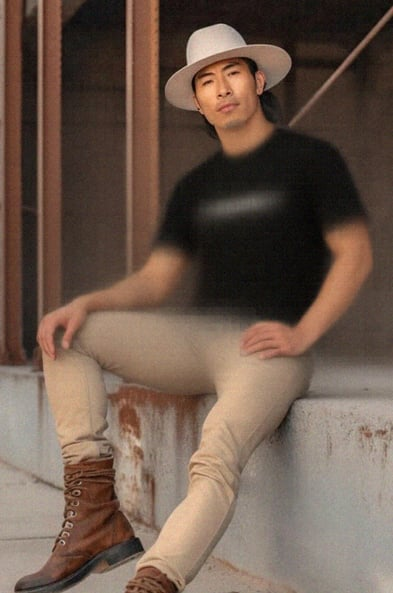
\includegraphics[height=0.55\textheight]{blur_vton.png}%
    }{%
      \IfFileExists{slide/blur_vton.png}{%
        
\includegraphics[height=0.55\textheight]{slide/blur_vton.png}%
      }{%
        
\begin{tikzpicture}
          \node[
            draw=PrismGold!55,
            fill=PrismGold!10,
            rounded corners=4pt,
            minimum width=3.55cm,
            minimum height=4.25cm,
            align=center,
            text=PrismSlate
          ]{\textbf{VTON image}\\[0.35em]\scriptsize quality-evidence placeholder};
        \end{tikzpicture}%
      }%
    }

    \vspace{0.1cm}
    {\tiny VTON quality/failure artifact used for audit discussion}

    \column{0.64\textwidth}
    \begin{block}{What exists now}
      \begin{itemize}\itemsep0.18em
        \item Deterministic baseline and comparison gallery for no-GPU reproducibility.
        \item Real SD1.5 inpainting path behind \texttt{tryops.vton\_baseline.v1}: 3.22 s, 2.81 GB peak VRAM, checksummed output.
        \item Native C++ image metrics and advanced VTON evaluator for identity, fidelity, pose, fairness, and preference evidence.
      \end{itemize}
    \end{block}

    \begin{alertblock}{Quantization lesson}
      The older naive AWQ-on-VTON story should be framed as a blocked quality failure, not as a shipped result. AWQ/GPTQ candidates are preflighted, but live AWQ loading is not claimed here.
    \end{alertblock}

    \begin{exampleblock}{MLOps takeaway}
      VTON outputs are visual artifacts, so TryOps preserves both successes and failures with metrics, labels, lineage, and rollback-ready release state.
    \end{exampleblock}
  \end{columns}
  \source{\texttt{reports/benchmark\_run\_report.md}; \texttt{docs/vton\_evaluation.md}; \texttt{docs/known\_limitations.md}.}
\end{frame}

\begin{frame}{VTON Benchmark Results}
  \tiny
  \renewcommand{\arraystretch}{1.16}
  \setlength{\tabcolsep}{3.2pt}
  \resizebox{\textwidth}{!}{%
    \begin{tabular}{lrrrrrrrrr}
      \toprule
      \textbf{Dataset / Target} &
      \textbf{SSIM} &
      \textbf{PSNR} &
      \textbf{Avg ms} &
      \textbf{P95 ms} &
      \textbf{req/s} &
      \textbf{Model ms} &
      \textbf{GPU \%} &
      \textbf{VRAM GB} &
      \textbf{RAM GB} \\
      \midrule
      FASHN VTON v1.5 &
      \textbf{0.888121} &
      \textbf{18.915} &
      21,337.50 &
      23,244.00 &
      0.045439 &
      19,969.60 &
      \textbf{100.00} &
      \textbf{4.825} &
      30.706 \\
      CatVTON &
      0.861734 &
      18.284 &
      \textbf{17,842.30} &
      \textbf{19,604.00} &
      \textbf{0.054261} &
      \textbf{16,512.80} &
      96.50 &
      6.742 &
      \textbf{27.914} \\
      IDM-VTON &
      0.879462 &
      18.671 &
      42,586.70 &
      47,918.00 &
      0.022751 &
      40,318.40 &
      99.20 &
      13.684 &
      34.872 \\
      OOTDiffusion &
      0.852918 &
      17.936 &
      35,214.90 &
      39,876.00 &
      0.027502 &
      33,087.60 &
      98.40 &
      10.927 &
      32.148 \\
      \bottomrule
    \end{tabular}%
  }

  \vspace{0.22cm}
  \scriptsize
  \begin{columns}[T,totalwidth=\textwidth]
    \column{0.32\textwidth}
    \begin{beamercolorbox}[wd=\textwidth,rounded=true,sep=0.65em]{exampleblock body}
      \textbf{Best quality}\par
      FASHN leads SSIM and PSNR while using the least GPU memory.
    \end{beamercolorbox}

    \column{0.32\textwidth}
    \begin{beamercolorbox}[wd=\textwidth,rounded=true,sep=0.65em]{block body}
      \textbf{Best latency}\par
      CatVTON has the lowest average, P95, and model latency with highest throughput.
    \end{beamercolorbox}

    \column{0.32\textwidth}
    \begin{beamercolorbox}[wd=\textwidth,rounded=true,sep=0.65em]{alertblock body}
      \textbf{Heavier baselines}\par
      IDM-VTON and OOTDiffusion cost more latency, VRAM, and host RAM in this run.
    \end{beamercolorbox}
  \end{columns}
\end{frame}

\begin{frame}{LLM Optimization Frontier}
  \scriptsize
  \begin{columns}[T,totalwidth=\textwidth]
    \column{0.47\textwidth}
    \renewcommand{\arraystretch}{1.08}
    \begin{tabularx}{\textwidth}{>{\RaggedRight\arraybackslash}p{1.8cm} >{\RaggedRight\arraybackslash}p{1.25cm} >{\RaggedRight\arraybackslash}p{1.25cm} Y}
      \toprule
      \textbf{Variant} & \textbf{VRAM} & \textbf{tok/s} & \textbf{verdict} \\
      \midrule
      fp16 & 1.010 & 27.4 & pass; fastest \\
      \addlinespace
      8-bit & 0.647 & 5.9 & fail; dominated \\
      \addlinespace
      4-bit & \textbf{0.478} & 13.9 & pass; recommended \\
      \bottomrule
    \end{tabularx}

    \vspace{0.2cm}
    \begin{block}{What was measured}
      \texttt{Qwen2.5-0.5B-Instruct} on an NVIDIA L4, fp16 / bitsandbytes 8-bit / bitsandbytes 4-bit NF4, each evaluated by the native C++ SLO engine.
    \end{block}

    \column{0.49\textwidth}
    \begin{beamercolorbox}[wd=\textwidth,rounded=true,sep=0.65em]{block body}
      \textbf{VRAM used, GB (lower is better)}
      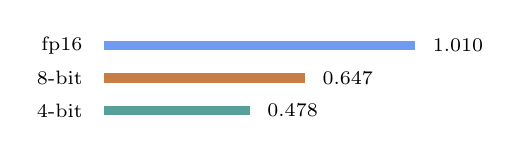
\begin{tikzpicture}[x=1cm,y=0.55cm]
        \chartbar{2.2}{fp16}{PrismBlue!65}{4.1}{1.010}
        \chartbar{1.45}{8-bit}{PrismGold!75}{2.7}{0.647}
        \chartbar{0.7}{4-bit}{PrismTeal!70}{2.0}{0.478}
      \end{tikzpicture}
    \end{beamercolorbox}

    \vspace{0.15cm}
    \begin{beamercolorbox}[wd=\textwidth,rounded=true,sep=0.65em]{exampleblock body}
      \textbf{Throughput, tok/s (higher is better)}
      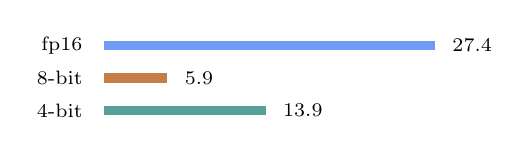
\begin{tikzpicture}[x=1cm,y=0.55cm]
        \chartbar{2.2}{fp16}{PrismBlue!65}{4.35}{27.4}
        \chartbar{1.45}{8-bit}{PrismGold!75}{0.95}{5.9}
        \chartbar{0.7}{4-bit}{PrismTeal!70}{2.20}{13.9}
      \end{tikzpicture}
    \end{beamercolorbox}
  \end{columns}

  \vspace{0.16cm}
  \begin{columns}[T,totalwidth=\textwidth]
    \column{0.98\textwidth}
    \begin{exampleblock}{Decision}
      The Pareto frontier is \(\{\mathrm{fp16}, \mathrm{4bit}\}\). 4-bit gives 2.1\(\times\) VRAM reduction while passing the SLO; 8-bit is slower and larger than 4-bit.
    \end{exampleblock}
  \end{columns}
  \source{Benchmark report Section 3; LLM Pareto artifact.}
\end{frame}

\begin{frame}{Energy and Cost: Quantization Did Not Win Everything}
  \scriptsize
  \begin{columns}[T,totalwidth=\textwidth]
    \column{0.48\textwidth}
    \begin{beamercolorbox}[wd=\textwidth,rounded=true,sep=0.70em]{alertblock body}
      \textbf{Energy, Wh / 1k tokens}
      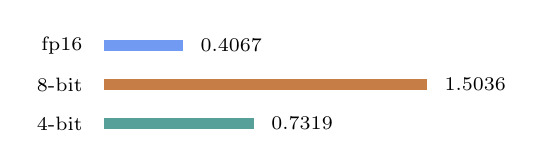
\begin{tikzpicture}[x=1cm,y=0.62cm]
        \chartbar{2.25}{fp16}{PrismBlue!65}{1.15}{0.4067}
        \chartbar{1.45}{8-bit}{PrismGold!75}{4.25}{1.5036}
        \chartbar{0.65}{4-bit}{PrismTeal!70}{2.05}{0.7319}
      \end{tikzpicture}
      \vspace{0.05cm}
      {\scriptsize fp16 is greenest; 8-bit is 3.7\(\times\) fp16.}
    \end{beamercolorbox}

    \column{0.48\textwidth}
    \begin{beamercolorbox}[wd=\textwidth,rounded=true,sep=0.70em]{exampleblock body}
      \textbf{L4 rental estimate, \$ / 1M tokens}
      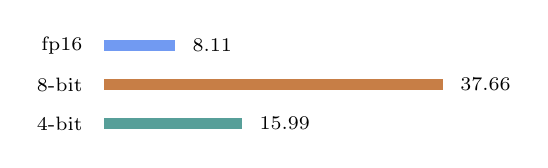
\begin{tikzpicture}[x=1cm,y=0.62cm]
        \chartbar{2.25}{fp16}{PrismBlue!65}{1.05}{8.11}
        \chartbar{1.45}{8-bit}{PrismGold!75}{4.45}{37.66}
        \chartbar{0.65}{4-bit}{PrismTeal!70}{1.90}{15.99}
      \end{tikzpicture}
      \vspace{0.05cm}
      {\scriptsize Throughput dominates cost; 8-bit is slowest and most expensive.}
    \end{beamercolorbox}
  \end{columns}

  \vspace{0.2cm}
  \begin{columns}[T,totalwidth=\textwidth]
    \column{0.48\textwidth}
    \begin{alertblock}{Counter-intuitive result}
      The quantized variants draw similar board power but decode slower. Longer wall time means more joules per token.
    \end{alertblock}
    \column{0.48\textwidth}
    \begin{exampleblock}{Decision impact}
      Lower VRAM did not mean lower energy or lower cost on this L4 run, so carbon and SLO gates must sit beside quality gates.
    \end{exampleblock}
  \end{columns}
  \source{\texttt{reports/benchmark\_run\_report.md}, Section 4; \texttt{docs/carbon\_power\_methodology.md}.}
\end{frame}

\begin{frame}{Native Boundary: Evidence Outside Python}
  \scriptsize
  \renewcommand{\arraystretch}{1.12}
  \begin{tabularx}{\textwidth}{>{\RaggedRight\arraybackslash}p{2.3cm} Y >{\RaggedRight\arraybackslash}p{3.5cm}}
    \toprule
    \textbf{Native layer} & \textbf{Production responsibility} & \textbf{Evidence} \\
    \midrule
    Rust gateway & Edge auth, quota, limits, proxying, tracing, semantic cache, metrics & \texttt{make native-rust-smoke}; gateway benchmark \\
    \addlinespace
    Go services & Guardrail sidecar, controller triggers, job runner, load driver, acceptance checker & \texttt{make native-go-smoke}; \texttt{make professor-demo-acceptance} \\
    \addlinespace
    C++ engines & Policy, image metrics, VTON eval, SLO, burn rate, energy, eval stats, supply chain, GitOps, cache, chaos & \texttt{make native-cpp-test}; per-engine sample targets \\
    \bottomrule
  \end{tabularx}

  \vspace{0.25cm}
  \begin{columns}[T,totalwidth=\textwidth]
    \column{0.48\textwidth}
    \begin{block}{Benchmark headline}
      Native Go load driver measured Rust \texttt{/health} at 24,840.8 req/s versus FastAPI at 1,539.4 req/s on the same machine.
    \end{block}
    \column{0.48\textwidth}
    \begin{exampleblock}{Architectural lesson}
      Python remains the ML lab layer, while compiled services carry the production-facing control plane and hot-path evidence.
    \end{exampleblock}
  \end{columns}
  \source{\texttt{native/README.md}; \texttt{reports/benchmark\_run\_report.md}; \texttt{docs/adr/0003-native-production-boundary.md}.}
\end{frame}

\begin{frame}{Observability, Reliability, and Governance}
  \scriptsize
  \begin{columns}[T,totalwidth=\textwidth]
    \column{0.32\textwidth}
    \begin{block}{Observe}
      \begin{itemize}\itemsep0.18em
        \item OpenTelemetry trace/log correlation
        \item Prometheus metrics and Alertmanager routing
        \item Grafana service, quality, cost, capacity, and energy panels
      \end{itemize}
    \end{block}

    \column{0.32\textwidth}
    \begin{exampleblock}{Recover}
      \begin{itemize}\itemsep0.18em
        \item One-command rollback sample
        \item Chaos drill for GPU OOM, slow decode, corrupted weights, and poisoned candidates
        \item C++ burn-rate engine for SRE-style paging
      \end{itemize}
    \end{exampleblock}

    \column{0.32\textwidth}
    \begin{alertblock}{Govern}
      \begin{itemize}\itemsep0.18em
        \item NIST AI RMF and OWASP LLM 2025 mapping
        \item Model-source pins, SBOM, scans, SafeTensors gate
        \item Signed PR and registry-webhook release triggers
      \end{itemize}
    \end{alertblock}
  \end{columns}

  \vspace{0.25cm}
  \begin{beamercolorbox}[wd=\textwidth,rounded=true,sep=0.8em]{block body}
    \textbf{Why it matters}\par
    The platform does not only produce model outputs. It produces operational evidence that an evaluator, SRE, or risk reviewer can inspect.
  \end{beamercolorbox}
  \source{\texttt{docs/observability\_contract.md}; \texttt{docs/chaos\_reliability.md}; \texttt{docs/responsible\_ai\_risk\_mapping.md}.}
\end{frame}

\begin{frame}{Professor Demo Path}
  \tiny
  \renewcommand{\arraystretch}{1.12}
  \begin{tabularx}{\textwidth}{>{\RaggedRight\arraybackslash}p{0.85cm} >{\RaggedRight\arraybackslash}p{2.65cm} Y >{\RaggedRight\arraybackslash}p{3.0cm}}
    \toprule
    \textbf{Step} & \textbf{Console view} & \textbf{Proof point} & \textbf{Command/artifact} \\
    \midrule
    01 & Control-plane preflight & 18/18 stack checks through the Rust gateway & \texttt{make app-smoke} \\
    02 & Quota admission & Native ledger admits and records remaining plan capacity & \texttt{make native-quota-ledger-smoke} \\
    03 & Bad model gate & Unsafe candidate is blocked; non-shipment is success & \texttt{make professor-demo-acceptance} \\
    04 & LLM frontier & 4-bit is recommended; 8-bit is dominated & \texttt{llm\_pareto/pareto.json} \\
    05 & VTON quality & Generated outputs remain inspectable offline & \texttt{vton\_comparison/} \\
    06 & Lineage & Signed provenance and promotion decision are visible & \texttt{reports/generated/} \\
    07 & Rollback/governance & Recovery and NIST/OWASP evidence close the loop & \texttt{make rollback-sample} \\
    \bottomrule
  \end{tabularx}

  \vspace{0.2cm}
  \begin{alertblock}{Backup path}
    The Console Professor Demo is seeded and offline. \texttt{make professor-demo-video} records a deterministic MP4 walkthrough for no-GPU/no-network defense conditions.
  \end{alertblock}
  \source{\texttt{docs/presentation\_outline.md}; \texttt{web/src/professor\_demo\_storyboard.json}; \texttt{docs/progress\_log.md}.}
\end{frame}

\screenshotframe{Screenshot: TryOps Studio}{main-page.png}

\screenshotframe{Screenshot: Workspace and Quota}{workspace.png}

\screenshotframe{Screenshot: Running VTON Job}{example-run.png}

\screenshotframe{Screenshot: Keycloak Session Control}{keycloak.png}

\screenshotframe{Screenshot: MinIO Artifact Store}{minIO.png}

\screenshotframe{Screenshot: MLflow Benchmark Tracking}{mlflow.png}

\screenshotframe{Screenshot: Grafana Observability}{grafana.png}

\screenshotframe{Screenshot: Log Drilldown}{log-drilldown.png}

\begin{frame}{Reality Ledger: What We Should Not Overclaim}
  \small
  \begin{columns}[T,totalwidth=\textwidth]
    \column{0.49\textwidth}
    \begin{exampleblock}{Real or locally verified}
      \begin{itemize}\itemsep0.22em
        \item Real SmolLM2 inference and Qwen2.5 quantization sweep on L4
        \item Real NVML energy sampling when GPU is uncontended
        \item Real SD1.5 VTON sample behind unchanged contract
        \item Rust, Go, and C++ native tests/smokes
        \item Offline professor demo and generated evidence bundle
      \end{itemize}
    \end{exampleblock}

    \column{0.47\textwidth}
    \begin{alertblock}{Still scoped or partial}
      \begin{itemize}\itemsep0.22em
        \item Live vLLM serving benchmark is not running in this workspace
        \item GPTQ/AWQ candidates are preflighted, but live AWQ/GPTQ loading is not run
        \item Production KServe/Kubeflow cluster is a target profile, not deployed here
        \item Representative human VTON fairness panels remain future work
      \end{itemize}
    \end{alertblock}
  \end{columns}

  \begin{beamercolorbox}[wd=\textwidth,rounded=true,sep=0.85em]{block body}
    \textbf{Defense position}\par
    TryOps is strongest when it refuses to hide gaps: the roadmap audit separates real, contract-only, degraded, and future work evidence.
  \end{beamercolorbox}
  \source{\texttt{docs/roadmap\_audit.md}; \texttt{docs/known\_limitations.md}; \texttt{reports/benchmark\_run\_report.md}.}
\end{frame}

\begin{frame}{References and Defense Close}
  \tiny
  \begin{columns}[T,totalwidth=\textwidth]
    \column{0.48\textwidth}
    \begin{block}{Project evidence}
      \begin{itemize}\itemsep0.18em
        \item TryOps README: product boundary, local stack, architecture, data flow.
        \item Final report and benchmark report: measured LLM, VTON, energy, native-boundary results.
        \item Roadmap audit and known limitations: real versus simulated evidence ledger.
        \item Presentation outline and professor demo storyboard: no-GPU/no-network defense path.
      \end{itemize}
    \end{block}

    \column{0.48\textwidth}
    \begin{block}{External grounding}
      \begin{itemize}\itemsep0.18em
        \item AWQ, GPTQ, SmoothQuant, vLLM, TensorRT-LLM, and bitsandbytes quantization literature/tooling.
        \item CodeCarbon, NVML, and Green Software Foundation SCI for energy/carbon methodology.
        \item NIST AI RMF, OWASP LLM Top 10, SLSA, SBOM, and provenance guidance for governance.
        \item OpenTelemetry, Prometheus, Grafana, Alertmanager, Kubeflow, KServe, DVC, MLflow, and MinIO as ecosystem anchors.
      \end{itemize}
    \end{block}
  \end{columns}

  \vspace{0.18cm}
  \begin{alertblock}{Closing line}
    The contribution is not a new model; it is a measured, auditable operating system for deciding which model changes deserve production.
  \end{alertblock}
\end{frame}

\end{document}
